\subsection{4-2-4 Encoder} 

%============================================================
\subsubsection{Two learning rate} 
\label{sec:tlr-auto4} 
\ref{sec:datasets-auto4} 
%======== (3D) L1 x L2 x epochs =========
%======== (3D) L1 x L2 x patSuccF =========
%TODO treat as main plot of the work 
\begin{figure}[H]
  \centering
  %TODO 10^glabels, same range, non-log epochs  
  \includegraphics[width=0.48\textwidth]{img/auto4_tlr_success.pdf}   
  \includegraphics[width=0.48\textwidth]{img/auto4_tlr_epoch.pdf}     
  \caption{TLR success and convergence on the \emph{4-2-4 Encoder} task with $\sigma = 2.3$ and $\mu = 0.0$.}
  \label{fig:results-tlr-auto4-performance}
\end{figure}

%======== (2D) best TLR on ALL_SUCC x epoch (std-dev) ==========
% TODO bitSucc, patSucc, F,B + std_dev 
\begin{figure}[H]
  \centering
  
\includegraphics[width=0.4\textwidth]{img/placeholder.png}    
  \caption{TLR success evolution for the \emph{4-2-4 Encoder} task.}
  \label{fig:results-tlr-auto4-epoch} 
\end{figure}

%============================================================
\subsubsection{Comparison} 
\ref{sec:datasets-auto4} 

For all our models \ref{sec:our-models} tested on the 4-2-4 encoder task~\ref{sec:datasets-auto4} TLR~\ref{sec:our-tlr} had the best success rate. 

For TLR, BAL, GeneRec, BP, CHL, other learning rules

\begin{table}
  \centering
    \begin{tabular}{|l|l|l|l|l|}
    \hline
    Algorithm&$\lambda$&Success&Epcs&SEM \\
    \hline
    BP&2.4&100&60&5.1\\
    \hline
    AP&2.8&100&54&3.6\\
    \hline
    GR&0.6&90&418&28\\
    \hline
    GR Sym&1.4&56&88&2.9\\
    \hline
    GR Mid&2.4&92&60&3.4\\
    \hline
    CHL&1.2&56&77&1.8\\
    \hline
    BAL&0.9&65&1000&\\
    \hline
    BAL TLR&0.0002 | 500&94&8251&\\
    \hline
    BAL Recirc&0.7&34&10000&\\
    \hline
    \end{tabular}
  \caption{Comparing performance of different models on the \emph{4-2-4 encoder} task.} 
  \label{tab:results-cmp-auto4}
\end{table}

TODO note that one epoch computation is not same for different models, for instance GeneRec needs to settle in the iterative approach 

%============================================================
\subsubsection{Hidden activations}
\ref{sec:our-hidden-activation}  

%===== TODO hidden activation timelines with commentaries (for TLR, BAL, GeneRec) 
% 2x success, 2x error (wrong settle, divergence) 

\begin{figure}[H]
  \centering
  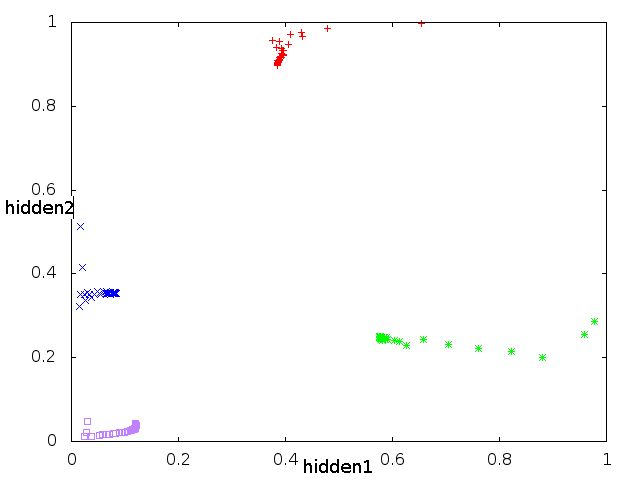
\includegraphics[width=0.45\textwidth]{../presentation/img/nice.png}   
  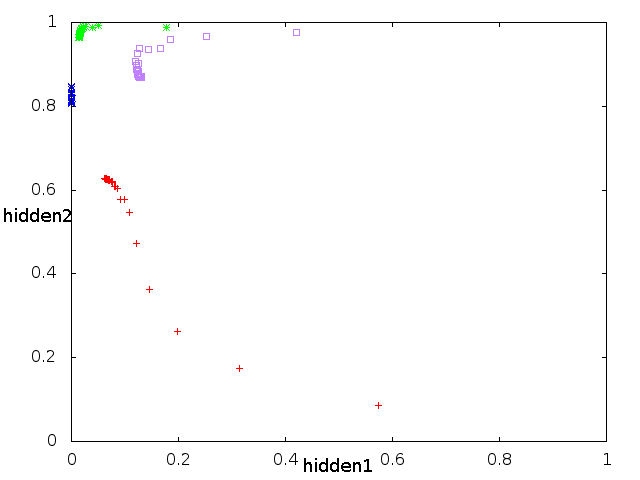
\includegraphics[width=0.45\textwidth]{../presentation/img/left_top.png}    
  \caption{BAL hidden activations on the \emph{4-2-4 encoder} for successfull networks.}
  \label{fig:results-hidden-activations-bal-good}
\end{figure}

\begin{figure}[H]
  \centering
  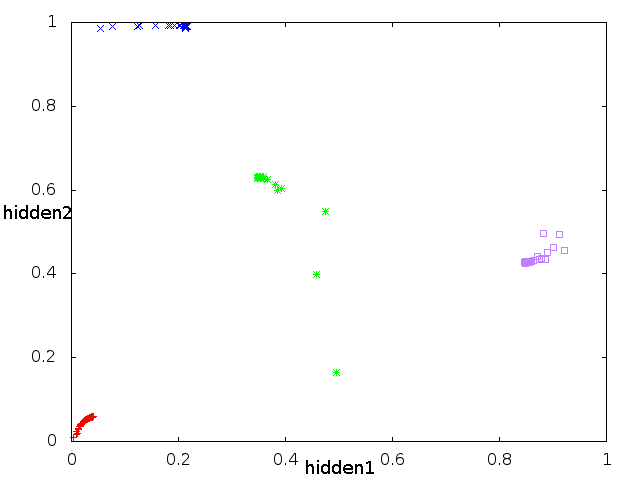
\includegraphics[width=0.45\textwidth]{../presentation/img/tazisko.png}   
  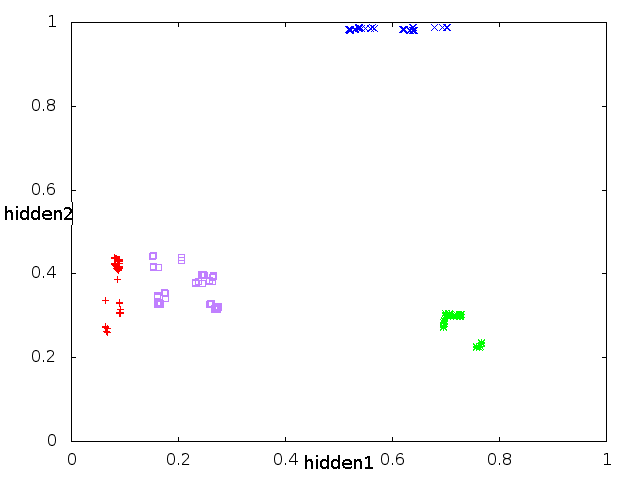
\includegraphics[width=0.45\textwidth]{../presentation/img/non-convergent.png}    
  \caption{BAL hidden activations on the \emph{4-2-4 encoder} for {\bf not} successfull networks. On the left image the network settled with constant hidden activations for which the resulting tw--dimensional task is not linearly separable. On the right image the network failed to convergence swtich several hidden activation states.}
  \label{fig:results-hidden-activations-bal-bad}
\end{figure}
